\chapter{Representação Tabular de Dados}
\section{Tabelas Estatísticas}

\inic Uma vez concluída a coleta e a ordenação dos dados de uma pesquisa, deve-se apresentá-los de tal forma que o leitor consiga identificar, rapidamente, uma série de informações, para tal, costuma-se utilizar inicialmente de uma tabela ou um quadro.\vskip0.3cm

\inic A representação tabular e uma apresentação numérica dos dados. Consiste em dispor os dados em linhas e colunas distribuídos de modo ordenado, segundo algumas regras práticas adotadas pelos diversos sistemas estatísticos. As regras que prevalecem no Brasil foram fixadas pelo Conselho Nacional de Estatística.\vskip0.3cm

\inic Uma tabela é um conjunto de dados estatísticos associados a um fenômeno, dispostos numa ordem de classificação, numa organização racional e prática de apresentação. A tabela resume ou sintetiza os dados, fornecendo o máximo de informação num mínimo de espaço.\vskip0.3cm

\inic Tabela é a forma não discursiva de apresentação de informações, representadas por dados numéricos e codificações, dispostos em uma ordem determinada, segundo as variáveis analisadas de um fenômeno.

\section{Por Que Tabelas São Importantes}

\inic Boas tabelas são parte integrante do seu pacote, seja um comunicado de imprensa, um artigo analítico ou um trabalho de pesquisa. O uso eficaz de tabelas ajuda a minimizar o número de valores de dados em seu texto. Também elimina a necessidade de discutir variáveis ​​menos significativas que não são essenciais para o enredo.\vskip0.3cm

As tabelas devem ser independentes, sejam elas publicadas em um relatório, artigo, publicação ou página da web. Cada tabela deve conter metadados suficientes, para permitir que ela seja copiada e colada em outro documento e ainda faça sentido.\vskip0.3cm

Se você garantir que suas tabelas possam ser independentes, é mais provável que elas sejam compreendidas corretamente, dentro ou fora de seu contexto original.

\subsection{Elementos  Básicos na Construção Tabular}

\inic Para a construção de uma série ou tabela estatística para que ela seja considerada dentro das normas de exposição. Estes elementos e regras são comuns a todas as tabelas. No Brasil, a apresentação tabular é regida pelas Normas de Apresentação Tabular do IBGE (1993) e NBR 14724 (ABNT, 2014).\vskip0.3cm


Os elementos básicos que constituem uma tabela são:

\begin{enumerate}
  \item \textbf{Número}: é utilizado para identificar a tabela no texto, onde as mesmas são numeradas a partir do número 1, como por exemplo: TABELA 1, TABELA 2, TABELA 3, etc, ou levando-se em consideração o capitulo do texto, como por exemplo, TABELA 1.1, TABELA 1.2, etc, para o capítulo 1, e, TABELA 2.1, TABELA 2.2 para o capítulo 2, e assim, sucessivamente.
  \item \textbf{Título}: Existem alguns mitos sobre o título de uma tabela, alguns autores relatam que, não existe título muito grande. Porém, no Brasil, basta seguir as regras definidas pelo (IBGE, 1993). Assim, o Título é uma designação que se coloca acima da tabela, ele deve ser preciso,
  indicando a natureza, local e época do evento, ou seja, explica o que a tabela contém e todo título deve responder as seguintes questões.

\begin{itemize}
  \item \textbf{O que $?$}  (Referente ao assunto a ser representado (\textbf{Fato}));
  \item \textbf{Como $?$}  (Referente as variáveis escolhidas para análise do fato (\textbf{Tipo}));
   \item \textbf{Onde $?$}   (Relativo ao lugar ou espaço geográfico onde ocorreu o fenômeno (\textbf{Local}));
    \item \textbf{Quando $?$} (Correspondente a época em que se verificou o fenômeno (\textbf{Tempo})).
\end{itemize}

O título deve ser escrito após o número da tabela, devendo ser separado do número por espaço, hífen e espaço, em letra maiúscula como o número. O título da tabela deve fornecer uma descrição clara e precisa dos dados, que seja curto e conciso e evite o uso de verbos.
\newpage
  \item \textbf{Cabeçalho}: parte superior da tabela (primeira linha) na qual é designada à natureza do conteúdo que especifica cada coluna. O cabeçalho pode ter um ou mais níveis. No primeiro nível o cabeçalho deve ser escrito preferencialmente em letras maiúsculas, enquanto que nos demais níveis somente a primeira letra deve ser maiúscula, sendo centralizado em cada coluna.
  \item \textbf{Corpo}: conjunto ou parte da tabela composta por linhas e colunas que contém as informações necessárias, formado pelo cabeçalho, coluna indicadora e numérica, onde o encontro ou cruzamento de uma linha e uma coluna é denominado casa, casela ou célula, sendo utilizado para observar as variáveis em esudo. 
  \item \textbf{Linhas}: Via de regra em pesquisas científicas, na linha são inseridos as respostas de uma pessoa, e nas colunas as variáveis ou características do evento. A linha é a parte do corpo da tabela que contém uma seqüência horizontal de informações.
  \item \textbf{Colunas}: A coluna é a parte do corpo que contém uma seqüência vertical de informações.
  \item \textbf{Casa ou Célula}: È o cruzamento de uma linha com a coluna, onde são indicados os dados e informações, sendo um espaço destinado a um só número.
  \item \textbf{Coluna Indicadora}: coluna que contém as discriminações correspondentes aos valores distribuídos pelas colunas numéricas, ou seja, é a primeira coluna que especifica o conteúdo de cada linha, devendo somente a primeira letra ser maiúscula, exceto quando se utilizarem de expressões que totalizam os dados como TOTAL, sendo alinhada a esquerda. Normalmente, se utilizam as categorias ou subcategorias das variáveis.
  \item \textbf{Rodapé}: É o espaço aproveitado em seguida ao fecho da tabela, reservado a observações pertinentes, onde são colocadas às notas de natureza informativa (fonte, notas, legendas, chamadas, etc).
  \item \textbf{Fonte}: refere-se à indicação das entidades ou órgãos responsável pela organização, origem, elaboração ou fornecimento dos dados expostos na tabela. A palavra fonte deve ser escrita em maiúscula seguida de dois pontos e espaço, seguindo o nome da fonte, sendo permitido o uso de siglas em letras maiúsculas. Deve ficar no rodapé da tabela. 
  \item \textbf{Notas}: São informações de natureza geral (indicados por algarismos romanos), onde o uso de notas, quando necessário, é destinado a esclarecimento (de forma geral ou específica) do conteúdo ou para indicar a metodologia utilizada na coleta dos dados. A palavra nota deve ser escrita em maiúscula seguida de dois pontos, no mesmo padrão do título, estando logo abaixo da fonte. Cada nota deve ser indicada em linha própria, podendo ou não ser numerada ou identificada por símbolos gráficos; As chamadas notas específicas servem para esclarecer minúcias em relação às casas, colunas ou linhas. São indicadas em algarismos arábicos ou símbolos gráficos;
  \item \textbf{Chamadas}: São informações de natureza específica (indicados por algarismos arábicos), colocados acima
  e à direita da coluna indicadora, nas demais colunas acima e a esquerda.
  Em suma, é um símbolo remessivo atribuído a algum elemento de uma tabela
  que necessita de uma nota específica.
\end{enumerate}


\begin{figure}[!htb]
\centering{
  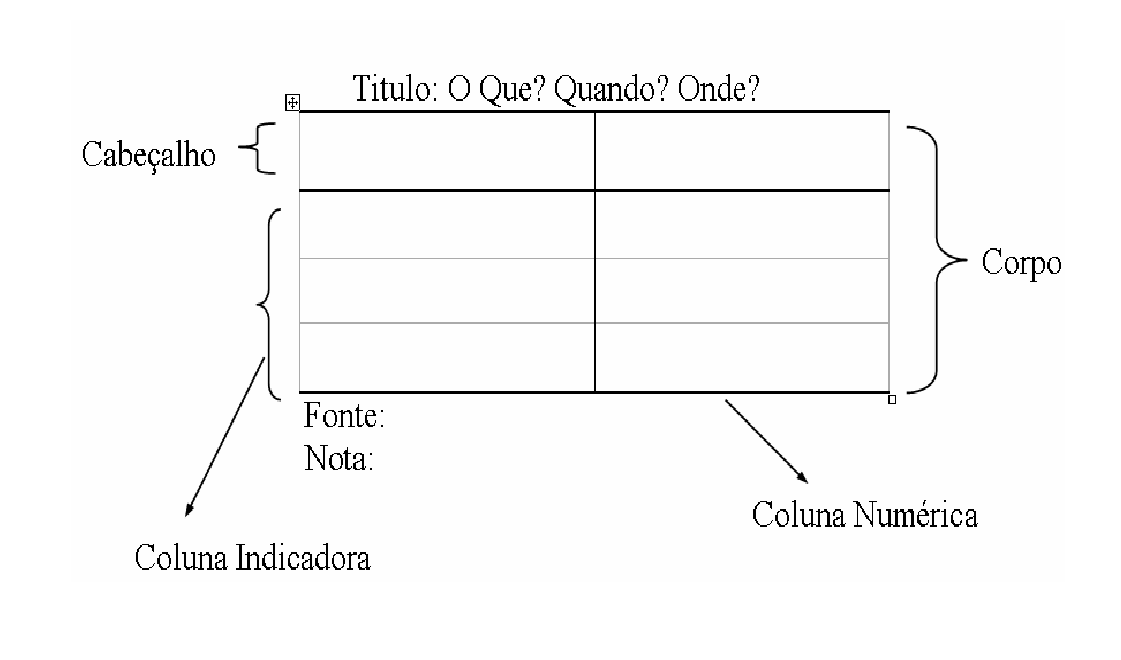
\includegraphics[scale=0.80]{figures/tab1.eps}\\
  \vspace{-0.8cm}
  \caption{Esquema Geral Sobre a Construção de uma
  Tabela conforme a NBR 14724 da ABNT de 2004.}\label{esquematabela1}}
\end{figure}



\newpage
Os valores dos dados devem ser definidos para que as informações principais possam ser extraídas facilmente. Os usuários podem achar mais fácil verificar colunas ou linhas, dependendo da sua mensagem. Você deve considerar isso ao decidir se deseja apresentar sua Tabela na orientação retrato ou paisagem. Linhas ou sombreamentos sutis também podem ser usados ​​para incentivar os usuários a ler horizontalmente, bem como verticalmente. O espaçamento e o sombreamento podem alterar a maneira como uma tabela é lida.




\subsection{Quadros Estatístico}

\inic Os quadros são definidos como arranjo predominante de palavras dispostas em linhas e colunas, com ou sem indicação de dados numéricos. È formado por linhas horizontais e verticais, sendo, portanto "fechado", e normalmente, é usado para apresentar dados secundários.\vskip0.3cm 

\inic Diferenciam-se das tabelas por apresentarem um teor esquemático e descritivo, e não estatístico. A apresentação dos quadros é semelhante à das tabelas, exceto pela colocação dos traços verticais em suas laterais e na separação das casas. Um quadro normalmente apresenta resultados qualitativos (textos). Pode usar espaçamento e fontes de letras com tamanhos menores que o do texto (não precisa seguir o mesmo padrão).   

\begin{quadro}[h!tp]
    \centering
    \caption{Equema geral sobre a construção um Quadro conforme as normas do IBGE de 1993}
    \begin{tabular}{|c|c|}
    \hline
    Cabeçalho  & Coluna indicadora   \\    
    \hline
           &           \\
           &              \\
           &              \\
           &              \\
           &              \\
           &              \\
           &              \\
  \hline
    \end{tabular}
\end{quadro}


\newpage

\inic Quando um relatório técnico possui tabelas  e Quadros, é necessário inserir uma Lista de Tabelas e Quadros de forma separada.



\subsection{Principais Recomendações para Construção Tabular}

\inic As normas adotadas neste livro, que fixam conceitos e procedimentos aplicáveis a elaboração de tabelas de dados numéricos, de modo a garantir a clareza das informações são apresentadas a seguir (IBGE, 1993)


\begin{enumerate}
\item Quanto a apresentação as tabelas podem ser intercaladas no texto, e imediatamente após o trecho que são citados pela primeira vez, de maneira que sua visualização tenha sentido normal de leitura;  
\item Toda tabela deve ter significado próprio, ou seja, suficientemente completa para ser entendida, dispensando consultas ao texto; 
\item Recomenda-se que uma tabela seja elabora
de forma a ser apresentada em uma única página.
\item Toda tabela contenha somente os dados necessários ao seu entendimento;
\item Inclua os dados logicamente ordenados e apresente dados, unidades e símbolos consistentes com o texto;
\item As tabelas podem ser apresentadas em anexo quando a quantidade de tabelas for grande ou quando ocupar mais de uma página, o que dificultaria a leitura do texto; 
\item Durante a representação em tabelas não se deve ter repetidos seus dados em gráficos ou figuras. Optar por um deles, sem perder de vista o que se quer comunicar, se os valores exatos ou aspecto visual, evitando assim, uma ambiguidade de informações;
\item Deve ter numeração independente e consecutiva; 
\item As tabelas devem ser colocadas em posição vertical para facilitar a leitura das informações, caso a tabela ultrapasse as margens, é necessário rotacionar a tabela. Lembrando que, na maioria dos relatórios, quando a tabela ultrapassa as margens, os autores diminuem a fonte para caber em mesma página, cometendo um erro gráfico e estético comum; 
\item Caso a tabela não couber em uma folha,
continuará na folha seguinte e, nesse caso, não é delimitada por
um traço horizontal na parte inferior, sendo o titulo e o
cabeçalho repetido na folha seguinte; 
\item Recomenda-se não
delimitar (fechar) por traços verticais, os extremos da tabela, à
direita e a esquerda, pois, assim, a mesma se torna um quadro;
\item As tabelas, excluídos os títulos, serão delimitadas, no alto e em baixo, por traços horizontais grosso preferencialmente;
\item Devem ser alinhadas de acordo com as margens do texto. O espaço entre as tabelas e texto deve ser de duas entrelinhas;
\item Usa-se um traço horizontal (-) hífen quando o dado for nulo, inexisti o fenômeno; 
\item Usa-se (...) reticência quando não se dispuser dos dados,
embora ele possa ser quantificado; 
\item Usa-se zero (0) quando o
valor é muito pequeno para ser expresso pela unidade utilizada.
\item Caso os dados sejam secundários, as fontes são obrigatórias.
\item Devem preferencialmente ser apresentadas no mesmo tipo e tamanho de letras adotados no texto ou reduzidas até um limite que não prejudique a sua leitura. Nunca em tamanho maior que o texto;
\item Não utilizar mais casas decimais do que o necessário para
não mascarar as comparações de interesse. 
\item Proponha um título
autoexplicativo e inclua as unidades de medidas. O título deve
dizer o que representam os números do corpo da tabela e, em geral,
não deve conter informações que possam ser obtidas diretamente dos
rótulos de linhas e colunas. 
\item Colocar os totais de linhas
e/ou colunas para facilitar as comparações. 
\item Ordene colunas
e/ou linhas quando possível. Se não houver impedimentos, ordene-as
segundo os valores, crescentes ou decrescentes. 
\item Tente trocar
de orientação (linhas por colunas) para melhorar a apresentação,
pois, é mais fácil fazer comparações ao longo das linhas do que
das colunas. 
\item Altere a disposição e o espaçamento das linhas
e colunas para facilitar a leitura. 
\item Não analise a tabela
descrevendo-a, mas sim, comentando as principais tendências
sugeridas pelos dados. 
\item È facultativo o emprego de traços
verticais para separação das colunas no corpo da tabela. 
\item
Quando uma tabela, por exessiva altura, tiver de ocupar mais de
uma página, 
\textbf{Não} deve ser delimitada na parte inferior,
repetindo-se o cabeçalho na página seguinte. Neste Caso, deve-se
usar, no alto no cabeçalho ou dentro da coluna indicadora a
designação continua ou conclusão, conforme o caso. 
\item Quando
uma tabela ocupar páginas confrontantes todas as linhas devem ser
numeradas na primeira e na ultima coluna. 
\item Quando não for
conveniente a apresentação de uma tabela em páginas confrontantes,
deverá a mesma ser dividida em duas ou mais. 
\item Se o disposto
no item anterior se tornar impraticável, por serem as colunas
insuscetíveis de agrupamento, deve-se desmenbrar a tabela em
seções, estas dispostas umas abaixo das outras e separadas por um traço horizontal duplo. 
\item Quando uma tabela tiver poucas
colunas e muitas linhas, poderá ser disposta em duas ou mais
partes, lado a lado, separando-se as partes por um traço vertical
duplo.
\item As expressões que totalizam os dados devem ser destacadas em negrito ou letras maiúsculas. Ex: Total, Subtotal, TOTAL;
\item Nenhuma casa da tabela deve ficar em branco, apresentando sempre um número ou sinal.
\item Deve ser evitado o uso de siglas e abreviaturas que não sejam de uso corrente; quando necessárias devem ser grafadas por extenso como nota na tabela;
\item O cabeçalho deve ser centralizado na coluna, com a letra inicial da primeira palavra maiúscula. O uso de outras letras maiúsculas deve respeitar as regras gramaticais do idioma. É facultativo grafar o cabeçalho em negrito, desde que seja mantida uniformidade em todas as tabelas.
\item A indicação de número no cabeçalho deve ser feita pela letra N, em maiúscula, já convencionado na literatura internacional. A indicação do número relativo deve ser feita pelo seu respectivo símbolo.
\end{enumerate}




%%%%%%%%%%%%%%%%%%%%%%%%% TABELA  %%%%%%%%%%%%%%%%%%%%%%%%%%%%%%%%%%%%%%%%%%%%%%%%%%%

\begin{sidewaystable}
\centering
    {
\caption{Exemplo de Tabela Rotacionada devido a Ultrapassagem da Margem (Item 9) , referente a Frota de Veículos Registrados em alguns Municípios Paraenses em setembro de 2022.}
\label{tabelarotacionada}
    \vspace{0.2cm}
\begin{tabular}{l|c|c|c|c|c|c|c|c}
\hline
Municípios & Automóvel & Motocicleta & Caminhonete  & Camioneta & Caminhão  & ônibus & Trator & Total \\
\hline\hline
Belém      & 220.492  & 127.747      & 27.092       & 17.397    & 9.087     & 3.877  & 1.249  & 5.587 \\
Marabá     & 26.941   & 56.931       & 9.091        & 2.100  & 3.686     & 771      & 649    & 425    \\
Santarém   & 29.295   & 44.002       & 7.674        & 2.680  & 3.042     & 770      & 169    & 1.170  \\ 
Ananindeua & 57.418   & 41.666       & 6.966        & 3.429  & 4.494     & 1.601    & 904    & 749    \\  
Itaituba   & 5.798    & 24.724       & 2.976        & 432    & 1.100     & 145      & 99     & 179    \\  
Redenção   & 10.172   & 35.873       & 4.569        & 353    & 1.771     & 175      & 208    & 257    \\
Castanhal  & 19.899   & 36.172       & 4.240        & 998    & 2.860     & 441      & 537    & 302     \\
Tucuruí    & 7.112    & 17.799       & 2.072        & 447    & 915       & 209      & 92     & 141    \\
Altamira   & 10.693   & 37.980       & 4.795        & 752    & 2.032     & 689      & 95     & 331    \\
\hline
  Total    & 387.820  & 383.294      & 69.475      & 28.588 & 27.997    & 8.678    & 4.002  & 9.141   \\
\hline\hline 
\end{tabular}} 
\begin{flushleft}
Fonte: DETRAN-PA,2022. 
\end{flushleft}
\end{sidewaystable}
%%%%%%%%%%%%%%%%%%%%%%%%%%%%%%%%%%%%%%%%%%%%%%%%%%%%%%%%%%%%%%%%%%%%%%%%%%%%%%%%%%%%%%%%%%%%%%


\newpage


\section{Séries Estatísticas}

\inic Uma série estatística é um conjunto ou coleção de dados ordenados segundo uma característica comum, as quais servirão posteriormente para se fazer análises e inferências. Resumidamente, uma série é um conjunto de números associados a fenômenos dispostos em correspondência com critério de modalidade. Ou seja, uma série é uma forma de organização mais completa e requer certas regras de construção.\vskip0.3cm


\inic As séries estatísticas em geral são de natureza quantitativa sendo expressas em tabelas ou matrizes operacionais, nas quais os dados são distribuídos de maneira organizada através de textos e números e de acordo com um caráter que é passível de variação (CARVALHO e ARAUJO, 2008).\vskip0.3cm

Pode-se dizer que toda série é uma tabela, mas nem toda tabela é
uma série, pois esta exige homogeneidade, classificação, critérios
de modalidade, segundo: \textbf{Espécie}, \textbf{Local} ou
\textbf{Época}. \vskip0.3cm

As séries podem ser classificadas em \textbf{simples} ou \textbf{conjugadas}. As séries simples são aquelas que apresentam variação em apenas uma das modalidades (espécie, local e tempo). São tabelas com apenas uma entrada e possuem apenas duas colunas. As séries conjugadas apresentam variação em duas ou mais modalidades, ou seja, são tabelas com duas ou mais entradas.\vskip0.3cm

As séries também são divididas em:


\begin{itemize}
  \item \textbf{Séries Homógradas} : aquelas em que a variável descrita apresenta variação discreta ou descontínua. São séries homógradas a série temporal, a série geográfica e a série específica;
 \item \textbf{Séries Heterógradas} : aquelas nas quais o fenômeno ou o fato apresenta graduações ou subdivisões. Embora fixo, o fenômeno varia em intensidade. A Distribuição de freqüências é uma série heterógrada.
\end{itemize}

\newpage
\subsection{Séries Estatísticas do IBGE}

O Banco de Dados Séries Estatísticas e Séries Históricas tem por objetivo disseminar, para um público diversificado (instituições governamentais, setor privado, área acadêmica, estudantes, ONGs), informações provenientes de dados oficiais oriundos de pesquisas do IBGE, em sua maior parte, e de outras fontes governamentais. Ordenadas segundo um intervalo de tempo, essas informações constituem Séries Estatísticas Históricas sendo, em muitos casos, séries longas (períodos superiores a 20 anos). \vskip0.3cm

Tais Séries se caracterizam pela natureza socioeconômica e demográfica de suas informações e também por apresentarem os conceitos das variáveis envolvidas, bem como as mudanças que sofreram ao longo do período considerado, além da notificação, sempre quando for o caso, de alterações metodológicas na pesquisa geradora dos dados (IBGE, 2022).\vskip0.3cm

Os temas contemplados pelas Séries Estatísticas \& Séries Históricas reúnem um acervo de informações sobre a realidade brasileira em suas dimensões social (educação, habitação, trabalho, saúde, organização familiar), demográfica (características da população, dinâmica demográfica e indicadores demográficos) e econômica ( sistema de contas nacionais; índices de preços, de produção e de comércio; agropecuária) que, sem excluir os dados de anos recentes, cobrem períodos tão longos quanto possível (IBGE, 2022).





\newpage 
\subsection{Séries Temporal, Histórica, Cronológica, Evolutiva ou Marcha}

\inic È a série cujos dados estão dispostos em correspondência
com a \textbf{Època}, nesta série o elemento de variação é o \textbf{Tempo} (dia,
mês e ano), ou seja, varia a época, mas o local(fator geográfico) e o fenômeno (espécie)
permanecem constantes (fixos).


\begin{table}[!htb]
    \centering
    {
    \caption{Número de Veículos Registrados do Tipo Motocicleta no Estado do Pará, durante o período de 2010 a 2022.}
    \label{obitos}
    \vspace{0.1cm}
\begin{tabular}{c|c}
  \hline\hline
  % after \\: \hline or \cline{col1-col2} \cline{col3-col4} ...
  Anos   & Frota Registrada \\
  \hline\hline
  2010   & 387.262  \\
  2011   & 439.825 \\
  2012   & 536.180  \\
  2013   & 597.402  \\
  2014   & 673.202 \\
  2015   & 742.456 \\
  2016   & 793.977 \\
  2017   & 835.898 \\
  2018   & 876.258 \\
  2019   & 967.240 \\
  2020   & 1.080.574 \\
  2021   & 1.236.288 \\
  2022   & 1.048.627   \\
  \hline\hline
\end{tabular}}
\\
\hspace{-1.0cm}
Fonte: Detran-Pa, 2022.
\end{table}


Os dados de tempo apresentam alguns traços interessantes como tendências, comportamentos sazonais, variação intensa (volatilidade) e não-linearidade.\vskip0.3cm






\newpage

\subsection{Séries Geográfica, Territorial, Espacial ou de Localização}

\inic È a série cujos dados estão dispostos em correspondência com o \textbf{Local}, nesta série o elemento de variação é o \textbf{Lugar} (Bairro, Município, Estado), ou seja, varia o local, mas o tempo (época) e o fato (espécie) permanecem constantes (fixos).



\begin{table}[!htb]
    \centering
    {
    \caption{Top 10 do Ranking da Frota de Veículos Registrados no Estado do Pará, em 2022.}
    \label{obitos2}
    \vspace{0.1cm}
\begin{tabular}{c|l|c}
  \hline\hline
  % after \\: \hline or \cline{col1-col2} \cline{col3-col4} ...
  Ranking   & Municípios    & Frota Registrada  \\
  \hline\hline
  1º        & Belém         &  502.379 \\
  2º        & Ananindeua    &  164.503 \\
  3º        & Marába        &  138.232 \\
  4º        & Paruapebas    &  126.152 \\
  5º        & Santarém      &  123.785 \\
  6º        & Castanhal     &  92.878 \\
  7º        & Redenção      & 74.076  \\
  8º        & Altamira      & 68.085 \\
  9º        & Itaituba      & 54.323 \\
  10º       & Paragominas   & 47.282 \\
  \hline\hline
\end{tabular}}
\\
\hspace{-2.0cm}
Fonte: Detran-Pa, 2022.
\end{table}

\newpage

\subsection{Séries Específica, Especificativa, Categórica ou Qualitativa}

\inic È a série cujos dados estão dispostos em correspondência com a \textbf{Qualidade}, nesta série o elemento de variação é a espécie (município, bairro, UF, escola, etc.), ou seja, varia o fato (espécie), mas o tempo (época) e o local (lugar) permanecem constantes (fixos).


\begin{table}[!htb]
    \centering
    {
    \caption{Frota de Veículos Registrados no Município de Belém em 2022.}
    \label{obitos2}
    \vspace{0.1cm}
\begin{tabular}{l|c}
\hline\hline
% after \\: \hline or \cline{col1-col2} \cline{col3-col4} ...
\textbf{Tipos de Veículos}   & \textbf{Frota Registrada} \\
\hline\hline
Automóvel     &  243.149 \\
Motocicleta   &  143.320 \\
Caminhonete   &  31.780  \\
Motoneta      &  26.578  \\
Camioneta     &  19.822  \\
Caminhão      &  10.403   \\
Utilitário    &  8.035   \\
Reboque       &  7.665   \\ 
Ônibus        &  3.990   \\
Semi-Reboque  &  3.297   \\
Micro-ônibus  &  2.212   \\
Ciclomotor    &  1.343   \\
Triciclo      &  604     \\
Motor-Casa    &  83      \\
Side-Car      &  82      \\
Trator        &  16      \\
\hline\hline
\textbf{Total}         & \textbf{502.379}   \\
\hline\hline
\end{tabular}}
\\
\hspace{-0.5cm} Fonte: Detran-Pa, 2022.
\end{table}

%\newpage

%Fazendo uma síntese das caracteristicas das séries estatísticas,
%verifica-se, o que permanesse fixo e variável, conforme os tipos
%de tabelas.


%\begin{table}[!htb]
%    \centering
%    {
%    \caption{Síntese dos Tipos de Séries Estatisticas.}
%    \label{}
%    \vspace{0.1cm}
%\begin{tabular}{l||c||c||c}
%  \hline\hline
  % after \\: \hline or \cline{col1-col2} \cline{col3-col4} ...
%  Situação       & Temporal          & Geográfica       & Específica     \\
%  \hline\hline
%  Parte Variável &  Epoca            & Local            & Fenômeno      \\
%  Parte Fixa     &  Local e Fenomeno & Epoca e Fenomeno & Epoca e Local \\
%  \hline\hline
%\end{tabular}}
%\end{table}


\newpage
\subsection{Séries Mista, Composta, Conjugada, Dupla Entrada ou Cruzada}


\inic É comum, todavia, haver necessidade de apresentar, em uma única tabela, mais do que uma série. Quando as séries aparecem conjugadas, tem-se uma tabela de dupla entrada. Em uma tabela desse tipo são criadas duas ordens de classificação: uma horizontal (linha) e uma vertical (coluna).


\begin{table}[!htb]
\footnotesize
    \centering
    {
    \caption{Vítimas de Acidentes de Trânsito segundo a Gravidade e Condição no Estado do Pará no período de 2015 a 2016.}
    \label{obitos2}
    \vspace{0.2cm}
\begin{tabular}{l|c|c|c|c|c}
  \hline\hline
                  &  \multicolumn{5}{c}{Gravidade da Vítima} \\
  \cline{3-6}
  Condição da Vítima &      & \multicolumn{2}{c}{Fatal }& \multicolumn{2}{c}{Não Fatal}  \\
  \cline{3-6}
                     &      & 2020                      & 2021  & 2020     & 2021 \\
  \hline
  Pedestre           &      & 280                       & 161   & 1.846    & 1.099  \\
  Ciclista           &      & 87                        & 62    & 1.379    & 731    \\
  Motociclista       &      & 627                       & 374   & 6.639    & 4.424  \\
  Condutor           &      & 149                       & 81    & 746      & 754    \\
  Passageiro         &      & 325                       & 132   & 2.728    & 1.497  \\
  \hline\hline
  Total              &      & 1.468                     & 810   & 13.338   & 8.505  \\
   \hline\hline
\end{tabular}}
\\
\hspace{-0.5cm} Fonte: Detran-Pa, 2022.
\end{table}














\newpage
\subsection{Distribuição de Frequência}

\inic A distribuição de frequência E uma série estatística na qual a variável observada esta dividida em subintervalos do intervalo total observado e o tempo, a espécie e a região permanecem fixas.\vskip0.3cm

De forma geral, os dados podem ser classificados como:


\begin{itemize}
  \item \textbf{Dados Brutos} : são os dados originais, que ainda não se encontram prontos para análise, por não estarem numericamente organizados. (Também são conhecidos como Tabela Primitiva).
  \item \textbf{Rol} :são os dados brutos, organizados em ordem crescente ou decrescente.
  \item \textbf{Dados Discretos} : a variável é discreta quando assume valores em pontos da reta real.
  \item \textbf{Dados Contínuos} : a variável pode assumir, teoricamente, qualquer valor em certo intervalo da reta real.
  \item \textbf{Dados Tabelados Não Agrupados em Classes} : os valores da variável aparecem individualmente.
  \item \textbf{Dados Tabelados Agrupados em Classes} : os valores da variável não aparecem individualmente, mas agrupados em classes.
\end{itemize}


\subsection{Tabela Primitiva e Rol}


\inic A tabela em que os elementos não foram organizados numericamente chama-se tabela primitiva. Por exemplo, considere o levantamento de dados da estatura de 40 funcionários do Detran-PA lotados na agência sede no município de Belém em 2020 (variável X), cujos resultados, em centímetros, mostrados na tabela a seguir, estão colocados na seqüência como foram obtidos.


\begin{table}[!htb]
    \centering
    {
    \caption{Estatura dos Funcionários do DETRAN sede no muncípio de Belém em 2022.}
    \label{estatura}
    \vspace{0.2cm}
\begin{tabular}{c|c|c|c|c|c|c|c|c|c}
  \hline\hline
  166 & 160 & 161 & 150 & 162 & 160 & 165 & 167 & 164 & 160 \\
  162 & 161 & 168 & 163 & 156 & 173 & 160 & 155 & 164 & 168 \\
  155 & 152 & 163 & 160 & 155 & 155 & 169 & 151 & 170 & 164 \\
  154 & 161 & 160 & 172 & 153 & 153 & 156 & 158 & 158 & 161 \\
  \hline\hline
\end{tabular}}
\\
\hspace{-5.5cm} Fonte: DETRAN, 2022.
\end{table}

\newpage

O primeiro passo para a organização dos dados é ordená-los de forma crescente ou decrescente. A tabela assim organizada recebe o nome de \textbf{rol}.


\begin{table}[!htb]
    \centering
    {
    \caption{Rol dos Funcionários do DETRAN sede no muncípio de Belém em 2022.}
    \label{estatura2}
    \vspace{0.2cm}
\begin{tabular}{c|c|c|c|c|c|c|c|c|c}
  \hline\hline
  150 & 154 & 155 & 157 & 160 & 161 & 162 & 164 & 166 & 169 \\
  151 & 155 & 156 & 158 & 160 & 161 & 162 & 164 & 167 & 170 \\
  152 & 155 & 156 & 158 & 160 & 161 & 163 & 164 & 168 & 172 \\
  153 & 155 & 156 & 160 & 160 & 161 & 163 & 165 & 168 & 173 \\
  \hline\hline
\end{tabular}}
\\
\hspace{-6.5cm} Fonte: DETRAN, 2022.
\end{table}



A simples organização dos dados em um rol de ordem crescente já permite determinar diretamente o menor valor (x= 150 cm), o maior valor (x= 173 cm), o valor que mais ocorre (x= 160 cm), e a amplitude da variação (a distância entre o maior e o menor, x= 173-150= 23 cm).\vskip0.3cm


Uma maneira mais concisa de mostrar os dados do rol é apresentar cada seguido pelo número de vezes que ocorre, ao invés de repetí-los. O número de ocorrências de um determinado valor recebe o nome de freqüência. Por exemplo, a estatura de 155 cm ocorre 4 vezes que se escreve f(155)= 4; a estatura de 150 ocorre 1 vez ou f(150) = 1.\vskip0.3cm


A tabela que contém todos os valores com a sua freqüência recebe o nome de distribuição de freqüência. Veja abaixo uma distribuição de freqüência construída a partir do rol anterior (separada em 3 partes):

\begin{center}
\begin{table}[!htb]
    \centering
    {
    \caption{Frequências das Estatura dos Funcionários do DETRAN sede no muncípio de Belém em 2022.}
    \label{estatura2}
    \vspace{0.2cm}
\begin{tabular}{c|c}
\hline\hline
Estatura (cm) & Frequência \\
  \hline\hline
  150 & 1  \\
  151 & 1 \\
  152 & 1  \\
  153 & 1  \\
  154 & 1  \\
  155 & 1  \\
  156 & 1  \\
  157 & 1  \\
  \hline\hline
\end{tabular}}
\begin{tabular}{c|c}
\hline\hline 
Estatura (cm) & Frequência \\
  \hline\hline
  158 & 2  \\
  160 & 5 \\
  161 & 4  \\
  162 & 2  \\
  163 & 2  \\
  164 & 3  \\
  165 & 1  \\
  166 & 1  \\
  \hline\hline
\end{tabular}
\begin{tabular}{c|c}
\hline
Estatura (cm) & Frequência \\
  \hline\hline
  167 & 1  \\
  168 & 2 \\
  169 & 1  \\
  170 & 1 \\
  172 & 1 \\
  173 & 1 \\
  \hline\hline
  Total & 40 \\
  \hline\hline
\end{tabular}
\end{table}
\end{center}


\newpage 

Ainda assim, o processo exige muito espaço em especial quando o
número de valores da variável (n) aumenta. O mais razoável nestes
casos, em especial quando a variável é contínua, é agrupar os
valores por intervalos. Deste modo, ao invés de listar cada um dos
valores que ocorrem, listam-se os intervalos de valores e a
freqüência correspondente, isto é, ao invés de colocar 1 aluno com
150 cm, 1 aluno com 151 cm, etc., coloca-se 4 alunos entre 150 e
154 cm. Este intervalo é escrito como $150 \vdash 154$ (a variável
pode estar desde 150 inclusive até 154 exclusive), portanto
valores 150, 150.1, 151, 152, 153, 153.5, 153.99 estariam neste
intervalo, mas 154 não. Definindo o rol de acordo com intervalos,
tem-se a seguinte tabela :


\newpage

\begin{table}[!htb]
    \centering
    {
    \caption{Distribuição de Frequências dos funcionários do Detran-PA lotados na agência sede no município de Belém em 2022.}
    \label{estatura2}
    \vspace{0.2cm}
\begin{tabular}{c|c}
\hline\hline
Estatura (cm) & Frequência \\
  \hline\hline
  150 $\vdash$ 154 & 4  \\
  154 $\vdash$ 158 & 9 \\
  158 $\vdash$ 162 & 11  \\
  162 $\vdash$ 166 & 8  \\
  166 $\vdash$ 170 & 5  \\
  170 $\vdash$ 174 & 3  \\
  \hline\hline
  Total            & 40  \\
  \hline\hline
\end{tabular}}
\\
\hspace{-0.5cm}
Fonte: DETRAN-PA, 2022.
\end{table}


%\vskip0.3cm

Procedendo desta forma perde-se a informação detalhada das
estaturas, mas se ganha em simplicidade, pois a análise dos dados
fica simplificada. Examinando a tabela acima, podemos facilmente
verificar que a maioria dos alunos tem estaturas entre 154 e 166
cm e que uma minoria é menor que 154 cm ou maior que 170. Esta
análise não é imediata da tabela em que todos os valores são
listados. Por outro lado, se desejarmos saber quantos alunos tem
150 cm de altura, esta informação não estará disponível, pois
somamos os alunos de 150, 151, 152 e 153 cm numa única classe da distribuição de freqüência. Assim, é neessário um conhecimento mais detalhado de como construir uma distribuíção de frequência.


\newpage


\subsection{Elementos Básicos da Distribuição de Frequência}


\begin{enumerate}
  \item Convenções
  \begin{itemize}
    \item $\vdash$ Intervalo fechado à esquerda e aberto a direita: apenas o limite inferior pertence ao intervalo;
    \item $\dashv$ Intervalo aberto à esquerda e fechado a direita: apenas o limite superior pertence ao intervalo;
    \item $\vdash$ $\dashv$ Intervalo fechado em ambos os lados: os dois limites pertencem aos intervalos;
    \item $-$ Intervalo aberto em ambos os lados: os dois limites não pertencem aos intervalos.
  \end{itemize}
  \item \textbf{Limite Inferior da Distribuição de Freqüência (LI)}: é o valor a partir do qual são contadas as observações na distribuição de freqüências, ou seja, é o menor valor da distribuição de freqüência;
  \item \textbf{Limite Superior da Distribuição de Freqüência (LS)}: é o valor até o qual são contadas as observações na Distribuição de freqüências, ou seja, é o maior valor da distribuição de freqüência;
  \item \textbf{Amplitude Total da Distribuição de Freqüência (AT)}: é a diferença existente entre o maior e menor valor observado da distribuição de freqüência;

     $$ AT=LS-LI $$

  \item \textbf{Classes de uma Distribuição de Freqüência (K)}: são os subintervalos nos quais são contadas as observações da variável. O número de classes (k) pode ser calculado de várias maneiras diferentes, sendo abordados os dois principais métodos;\vskip0.3cm
\textbf{Método Prático 1}:

$$ k= 1+3,22 \ log \ n \Rightarrow \ Formula \ de \ Sturges $$

\textbf{Método Prático 2}: \vskip0.3cm

Se o número de elementos $n < 25$  utiliza-se o número de classes $k= 5$, se o número de componentes for
$n \geq 25$  utiliza-se o número de classe $k=\sqrt{n}$.
  \item \textbf{Limite Inferior da Classe (li)}: é o valor a partir do qual são contadas as observações dentro da classe, ou seja, o menor valor da classe;
  \item \textbf{Limite Superior da Classe (ls)}: é o valor até o qual são contadas as observações dentro da classe, ou seja, é o maior valor da classe;
  \item \textbf{Amplitude ou Intervalo de Classe (h)}: é o comprimento da classe, dado pela seguinte equação:
      \begin{equation}\label{}
        H=\frac{AT}{k}=\frac{(Maior \ Valor - \ Menor \ Valor)}{Numero \ de \ Classes}
      \end{equation}
  \item \textbf{Freqüências Simples ou Absolutas da Classe (fi)}: é o numero de observações contadas dentro de cada classe;
  \item \textbf{Freqüências Absolutas Acumulada da Classe (Fi)}: é a acumulação sucessiva, a partir da primeira classe até uma classe qualquer, das freqüências simples ou absoluta das classes;


      $$ F_{1}= f_{1} $$
      $$ F_{2}= f_{2} $$
      $$ \ldots  $$
      $$ F_{k}=  \sum_{i=1}^{j}f_{i} = f_{1}+f_{2}+\ldots+ f_{k}$$


  \item \textbf{Freqüências Relativas da Classe (fr)}: é a relação existente entre a freqüência absoluta ou simples de cada classe e o número de observações da variável, obtendo a partir da seguinte equação;

      \begin{equation}\label{}
        f_{r}=\frac{f_{i}}{\sum_{i=1}^{n}f_{i}}
      \end{equation}

Se as frequências da tabela forem substituídas pelas relativas correspondentes, a tabela resultante denomina-se \textbf{distribuição de frequência relativa}, \textbf{distribuição percentual} ou \textbf{tabela de frequências relativas}.\vskip0.3cm

As representações gráficas das distribuições de frequências relativa podem ser visualizadas utilizando o \textbf{Histograma} ou o \textbf{Polígono de Frequências}, mediante a simples modificação da escala vertical para as frequências relativas.



\item \textbf{Freqüências Relativas Acumuladas (Fr)}: é a acumulação sucessiva, a partir da primeira classe até uma classe qualquer das freqüências relativas das classes;

    $$ F_{r1}=f_{r1} $$
    $$ F_{r2}=f_{r2} $$
    $$   \ldots  $$
    $$ F_{rk}=  \sum_{i=1}^{j}f_{r_{i}}  = f_{r1}+f_{r2}+\ldots+ f_{rk}= \frac{f_{1}+f_{2}+\ldots+f_{j}}{n}$$

Uma tabela que apresenta frequências acumuladas denomina-se \textbf{distribuição de frequência acumulada}, \textbf{tabela de frequência acumulada} ou simplesmente \textbf{distribuição acumulada}.\vskip0.3cm

Um gráfico que apresenta a frequência acumulada abaixo que qualquer limite superior de classe, locada em relação a esse limite é denominado \textbf{Polígono de Frequência Acumulada} ou \textbf{Ogiva}




    \item \textbf{Ponto Médio da Classe (xi)}: é a média aritmética calculada entre o limite inferior e o superior de cada classe, a partir da seguinte fórmula.
\end{enumerate}


$$ x_{i}=\frac{ls+li}{2} $$


\subsection{Construção da Distribuição de Frequência}

\inic \textbf{Passo 1}: Colocar os dados em forma de Rol. Isto é, organizá-los de forma crescente ou decrescente. Aqui se recomenda colocá-los em ordem crescente.\vskip0.3cm

\textbf{Passo 2}: Identificar o valor máximo e o valor mínimo do conjunto de dados e encontrar a Amplitude Total (AT), sendo a diferença entre o maior $(x_{maximo})$ e o menor $(x_{minimo})$  valor observado no conjunto de dados:

$$ AT= x_{maximo}- x_{minimo} = ls - li$$

\textbf{Passo 3}: Determinar o número de classes (K) que irão formar uma distribuição de freqüências. Embora não exista uma forma precisa para esse número K, pode-se orientar a seguinte prática:


$$ k \cong \sqrt{n}$$


\textbf{Passo 4}: Calcular o comprimento ou a amplitude que deve ter o intervalo de classe (h), que e obtido dividindo-se a amplitude total pelo numero de classe, ou seja:


$$ h = \frac{AT=(ls-li)}{k}$$


\textbf{Passo 5}: Depois de organizados os dados, calculado o número e o intervalo de classes, partiu-se para a construção das classes.


\begin{itemize}
  \item $\textbf{1}^{ª}$ \textbf{classe}: Limite Inferior = menor valor do Rol\\
  Limite Superior = Limite Inferior da $1^{ª}$ classe + valor do intervalo de classe.
  \item $\textbf{2}^{ª}$ \textbf{classe}: Limite Inferior = Limite Superior da 1 classe\\
  Limite Superior = Limite Inferior da $2_{ª}$ classe + valor do intervalo de classe.
  \item \textbf{k classe}: Limite Inferior = Limite Superior da (k-1) classe\\
               Limite Superior = Limite Inferior da k classe + valor do intervalo de classe.
\end{itemize}



\textbf{Passo 6}: Depois de organizados os dados e construído as classes, obtêm-se as freqüências simples ou absolutas de cada classe ($f_{i}$).\vskip0.3cm

Assim, depois de seguido os seis passos, constrõem-se a distribuição de frequência, conforma a Tabela (3.9) utilizando dados reais.


\begin{table}[!htb]
    \centering{
    \caption{Esquema Geral para Construção de Distribuição de Frequência Tradicional.}
    \label{tox}
    \vspace{0.1cm}
\begin{tabular}{c|c|c|c}
  \hline\hline
          Classes                                        & $f_{(i)}$             & $f_{(r_{i})}$           & $\%$ \\
  \hline\hline
  $X_{min}   \hspace{1.7cm} |--- X_{min}+h  $           &  $n_{1}$               & $f_{1}=\frac{n_{1}}{n}$ & $100 \times f_{1} \%$ \\
  $X_{min}+h  \ \ \ \  \hspace{0.7cm}|--- X_{min}+2h $   &  $n_{2}$              & $f_{2}=\frac{n_{2}}{n}$ & $100 \times f_{2} \%$\\
  $X_{min}+2h \ \ \  \hspace{0.7cm} |--- X_{min}+3h $     &  $n_{3}$             & $f_{3}=\frac{n_{3}}{n}$ & $100 \times f_{3} \%$\\
      \vdots \vdots                                      &    \vdots \vdots      & $\vdots$                & $\vdots$ \\
  $X_{min}+(k-1)h \ \ |--- X_{min}+kh $                    &  $n_{k}$            & $f_{k}=\frac{n_{k}}{n}$ & $100 \times f_{k} \%$\\
  \hline\hline
  Total                                                  & $\sum_{i=1}^{k}n_{k}=n$ & $\sum_{i=1}^{k}f_{k}=1$ & $100 \%$\\
    \hline\hline
\end{tabular}}
\end{table}
\vskip0.1cm

\newpage

\textbf{Exemplo 1}: Considere uma amostra de 23 condutores abordados durante a operação lei seca, das
quais foram obtidas medidas de dosagem alcoólica pelo etilômetro (g).\vskip0.3cm


\begin{table}[!htb]
    \centering
    {
    \caption{Medidas de Dosagem Alcoólica de Etilômetros coletadas na Operação Lei Seca no Município de Belém em 2022.}
    \label{estatura}
    \vspace{0.2cm}
\begin{tabular}{c|c|c|c|c|c|c|c|c}
  \hline\hline
  0.77 & 0.75 & 0,80 & 0,78 & 0,75 & 0,65 & 1,02 & 0,75 & 0,55 \\
  0.85 & 0.61 & 0,78 & 0,58 & 0,52 & 0,78 & 1,10 & 0,65 &    \\
  0.85 & 0.90 & 0,96 & 0,79 & 0,55 & 1,05 & 0,99 & 0,75 &    \\
  \hline\hline
\end{tabular}}
\\
\hspace{-5.5cm}
Fonte: DETRAN-PA, 2022.
\end{table}

Os dados, como apresentado acima, são chamados brutos, pois ainda não foram submetidos a nenhum tipo de tratamento. Inicialmente, os dados devem ser colocados em ordem crescente (rol):


\begin{table}[!htb]
    \centering
    {
    \caption{Rol das medidas de dosagem Alcoólica de Etilômetros coletadas na Operação Lei Seca no município de Belém em 2022.}
    \label{estatura}
    \vspace{0.2cm}
\begin{tabular}{c|c|c|c|c|c|c|c}
  \hline\hline
  0,52 & 0,58 & 0,75 & 0,75 & 0,78 & 0,80 & 0,90 & 1,02 \\
  0,55 & 0,61 & 0,75 & 0,77 & 0,78 & 0,85 & 0,96 & 1,10  \\
  0,55 & 0,65 & 0,75 & 0,78 & 0,79 & 0,85 & 0,99 &     \\
  \hline\hline
\end{tabular}}
\end{table}


%\newpage 

Pode-se observar, agora, que das 25 observações o menor valor é $x_{minimo = 0,55}$ e o maior é $x_{maximo= 1,10}$. Para os dados acima, pode-se calcular a amplitude total $AT = x_{maximo}-x_{minimo}=1,10-0,52=0,58$
\\



Observe que esse exemplo contém um numero pequeno de observação (n=25), quando há um grande número de dados observados o processo de ordenação é trabalhoso e a listagem final pouco representará. Nesses casos, pode-se simplificar o processo agrupando os dados em certo número de classes, cujos limites serão denominados limite inferior e limite superior. A quantidade de classes e a amplitude destas devem ser obtidas observando as seguintes normas:


\newpage
\begin{itemize}
  \item As classes devem cobrir a amplitude total;
  \item O extremo superior de uma classe é o extremo inferior da classe seguinte;
  \item Cada valor observado deve enquadra-se em apenas uma classe;
  \item O número total de classes não deve ser inferior a 5 e nem superior a 25;
\end{itemize}


O número de classes (k), pode ser obtido de uma das fórmulas seguintes:

$$ k=\sqrt{n} \ \ \ \mbox{ou} \ \ \  k=1+3,22 \ log(n)$$



Para o exemplo, $k=\sqrt{25}=5$ ou $k=1-3,22 \ log(25)\cong 5,5$. Dividindo a amplitude total (AT) por k=5 chega-se ao tamanho ou amplitude de cada uma das classes: $h=\frac{AT}{k}=\frac{0,58}{5}=0,12$\vskip0.3cm


Quando os valores observados são números inteiros, os limites das classes também devem ser números inteiros. Para isso, aconselha-se escolher o número mais próximo de AT que resulte h em um número inteiro.\vskip0.3cm


Agora, utilizando esse valor pode-se obter os limites inferiores e superiores das classes:



\begin{itemize}
  \item o limite inferior da primeira classe pode ser o menor valor da série, neste caso 0,52;
  \item os demais limites serão obtidos somando aos limites inferiores o valor de h, isto é,
\end{itemize}

\begin{table}[!htb]
    \centering
    {
    \label{}
    \vspace{-0.5cm}
\begin{tabular}{l|c}
\hline\hline  
  $0,52 \vdash (0,52+ h=0,52+0,12)=$ & 0,64 \\
  $0,64 \vdash (0,64+ h)= \ldots $   & 0,76 \\
  $0,76 \vdash (0,76+ h)= \ldots $   & 0,88 \\
  $0,88 \vdash (0,88+ h)= \ldots $   & 1,00 \\
  $1,00 \vdash (1,00+ h)= \ldots $   & 1,12 \\
\hline\hline    
\end{tabular}}
\end{table}

\newpage

A partir da listagem ordenada das classes, pode-se construir
as chamadas tabelas de freqüência ou distribuição
de freqüência, que permitem uma melhor visualização dos dados.
Assim, no caso da amostra de 25 testes de dosagem alcoólica 
a distribuição de freqüência pode ser da seguinte forma:


\begin{table}[!htb]
    \centering
    {
    \caption{Distribuição de Frequência das Medidas de Medidas de Dosagem Alcoólica da Operação Lei Seca em Belém em 2022.}
    \label{toxalimentar}
    \vspace{-0.1cm}
\begin{tabular}{l|c}
  \hline\hline
  Dosagem Alcoólica (dg) & Frequência \\
  \hline\hline
  $0,52 \vdash 0,64$ & 5 \\
  $0,64 \vdash 0,76$ & 6 \\
  $0,76 \vdash 0,88$ & 8 \\
  $0,88 \vdash 1,00$ & 3 \\
  $1,00 \vdash 1,12$ & 2 \\
  \hline\hline
  Total & 25 \\
    \hline\hline
\end{tabular}}
\end{table}

\newpage

\section{Tabelas Bidimensionais}

È muito frequênte o interesse em verificar se duas variáveis
qualitativas apresentam-se associados, isto é, se o conhecimento de uma
variável ajuda a enterder uma outra variável.\vskip0.3cm


A representação geral de uma tabela bidimensional, também chamada como tabela de contingência
para as variáveis categóricas X e Y, com s e r categorias, respectivamente, construídas a partir de um conjunto de n elementos. As s categorias da variável X estão representadas por $X_{1},X_{2},\ldots,X_{s}$ e as r de Y por $Y_{1},Y_{2},\ldots,Y_{r}$ e suas combinações formam as $s \times r$ caselas ou células da tabela.


\begin{table}[!htb]
    \centering
    {
    \caption{Esquema Geral de Tabela Bidimensional}
    \label{Bidimensional}
    \vspace{0.2cm}
\begin{tabular}{l|c|c|c|c|c}
  \hline\hline
                     &  \multicolumn{4}{c}{Y} \\
  \cline{2-5}
  X                  & $Y_{1}$     & $Y_{2}$     & $\ldots$    & $Y_{r}$  & Total \\
  \hline
  $X_{1}$            & $ n_{11}$   & $ n_{12}$   & $\ldots$    & $n_{1r}$ & $n_{1.}$ \\
  $X_{2}$            & $ n_{21}$   & $ n_{22}$   & $\ldots$    & $n_{2r}$ & $n_{2.}$  \\
  $\vdots$           & $\vdots$    & $\vdots$    & $\ldots$    & $\vdots$ & $\vdots$ \\
  $X_{s}$            & $ n_{s1}$   & $ n_{s2}$   & $\ldots$    & $n_{sr}$ & $n_{s.}$ \\
  \hline\hline
  Total              & $n_{.1}$    & $n_{.2}$    & $\ldots$    & $n_{.r}$ & $n$ \\
   \hline\hline
\end{tabular}}
\end{table}


No corpo da tabela, $n_{11}$ é a frequência obeservada de
elementos que pertencem a categoria $X_{1}$ e $Y_{1}$
 simultaneamente. De um modo geral, $n_{ij}$ é a frequência observada de elementos que pertencem a categoria
 $X_{i}$ e $Y_{j}$ simultaneamente, com $i=1,2, \ldots,s $ e $j=1,2, \ldots ,r $. Os valores
 $n_{i.}=\sum_{j=1}^{r}n_{ij}$ , $n_{.j}=\sum_{i=1}^{s}n_{ij}$ e $n=n..=\sum_{i=1}^{s}\sum_{j=1}^{r}n_{ij}$
representam os totais das linhas, os totais das colunas e o total
geral, respectivamente.















